\chapter{SYSTEM ARCHITECTURE AND METHODOLOGY}

\section{System Block Diagram/Architecture}
\vspace{20pt}
\begin{figure}[H]
	\centering
	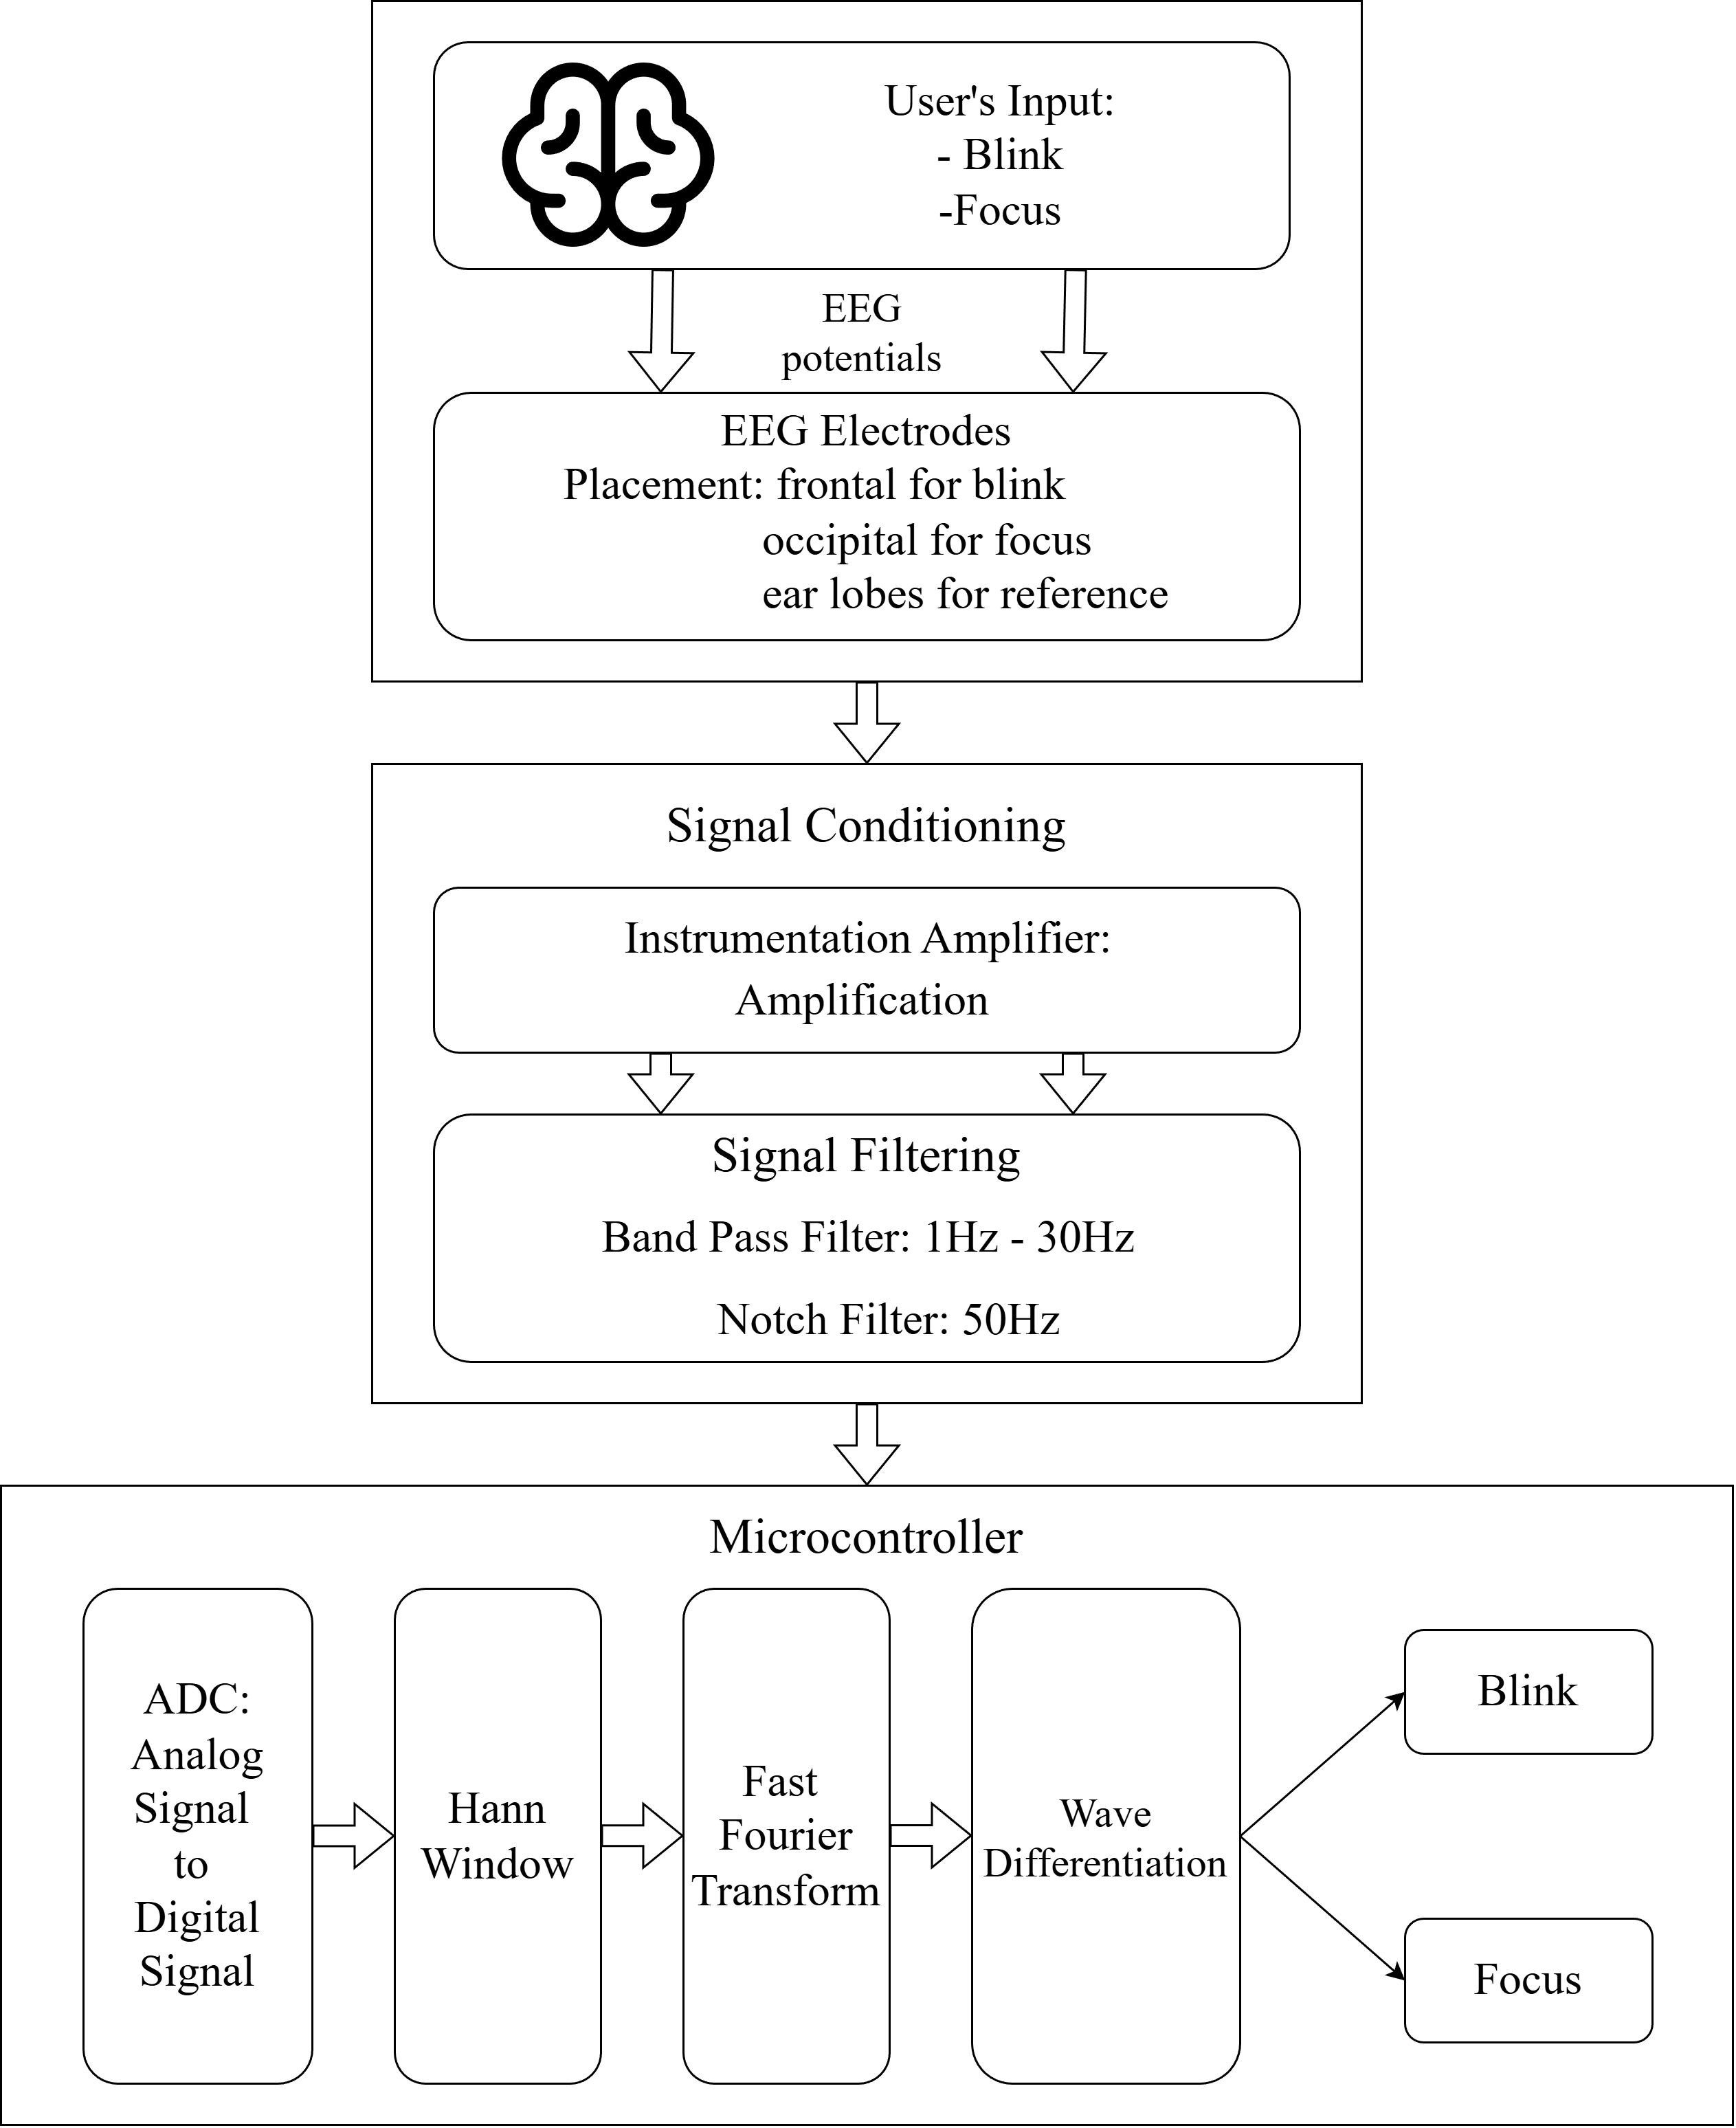
\includegraphics[width = 14.5cm, height=19.5cm]{src/images/figures/system_architecture.png}
\caption{System Block Diagram of the Brain-Computer Typing Interface}
\label{system_block_diagram}
\end{figure}

\newpage
\section{ Working Principle}
Brain Computer Interface (BCI) system is responsible for sensing, amplifying, filtering, and interpreting brain electrical signals for controlling external devices. EEG signals are sensed by electrodes attached to the scalp. The weak signals are amplified using Instrumentation Amplifier (AD620). Band pass filter such as Butterworth filter is used to filter out the required frequency signals and artifact as well as muscle activity.

Filtered signals are further converted into digital signals through ADC port of Arduino. Signal frequencies are analyzed using software algorithms that help in identifying visual stimuli that the user is concentrating on. This system is very sensitive, noise free and interference free.

More precisely, EEG electrodes are placed on the scalp at frontal and occipital regions to capture signals related to eye blinks and brain activity. A large voltage change appears in the EEG signal when the user performs an intentional eye blink. The proposed BCI typing system works by detecting eye blinks and changes in beta wave activity from EEG signals to control a typing or selection interface but beta wave activity varies depending on the user’s level of focus or relaxation and is mainly observed in the occipital region of the brain.

The EEG signals collected from the electrodes are first amplified and conditioned using an analog front end circuit then these signals are passed through analog filters including high pass and low pass to remove unwanted noise, baseline drift and power line interference. Then the clean EEG signals are converted into digital form using an analog to digital converter.

In the digital stage, the system stores the sampled EEG data in short time windows. Eye blinks are detected directly from the time domain signal using amplitude thresholding techniques and based on predefined thresholds, the system determines whether the user is focused or relaxed. For beta wave analysis, Fast Fourier Transform (FFT) is applied to the observed EEG data to calculate the power in the beta frequency band (12-30 Hz). If blink and beta states are detected then it is processed by a rule based decision logic, which translates them into typing or selection actions on the user interface.

\newpage
\section{Flowchart of Proposed System Architecture}
\vspace{18pt}
\begin{figure}[H]
	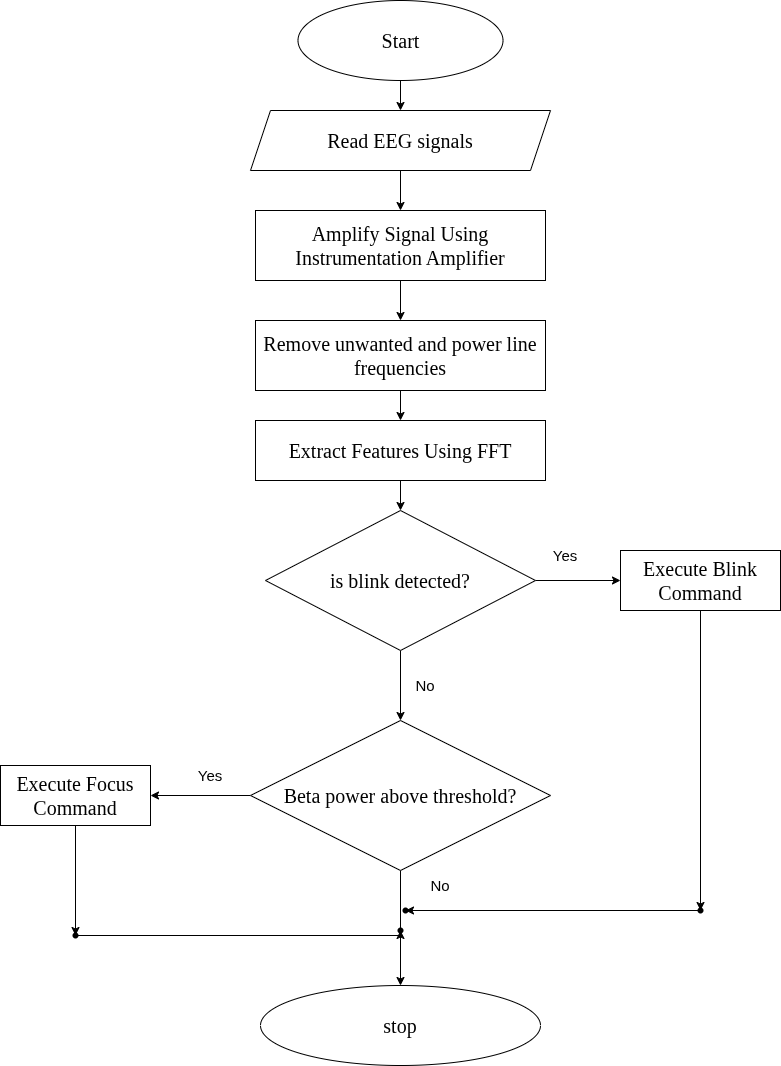
\includegraphics[width = 14cm, height = 21.5cm]{src/images/figures/flowchart.png}
	\vspace{10pt}
	\caption{Flowchart of Proposed System Architecture}
	\label{flowchart}
\end{figure}

\newpage
This flowchart illustrates the operation of the proposed EEG-based BCI system. The system acquires EEG signals, amplifies them using an instrumentation amplifier, and removes unwanted noise and power-line interference through filtering. FFT is then applied to extract relevant features. Based on these features, the system first checks for blink detection to execute a blink command; if no blink is detected, it evaluates beta-band power to determine focus and execute the corresponding focus command, after which the process ends.

\section{FFT flowchart for Arduino Program}
\tikzset{
	startstop/.style={
		ellipse,
		draw=black, thick,
		minimum width=5cm,
		minimum height=0.9cm,
		align=center,
		font=\small
	},
	process/.style={
		rectangle,
		draw=black, thick,
		minimum width=8cm,
		minimum height=1cm,
		align=center,
		font=\small,
		inner sep=6pt
	},
	decision/.style={
		diamond, aspect=3,
		draw=black, thick,
		minimum width=7cm,
		align=center,
		font=\small,
		inner sep=2pt
	},
	arrow/.style={-{Stealth[length=6pt]}, thick},
}
%% ════════════════════════════════════════════════════════
%%  PAGE 1 — Interrupt Service Routine
%% ════════════════════════════════════════════════════════
\begin{figure}[H]
	\centering
	\begin{tikzpicture}[node distance=0.65cm]
		
		\node (isrstart) [startstop]                        {Timer interrupt fires};
		\node (adc)      [process,  below=of isrstart]      {Start conversion\\read and scale raw sample};
		\node (wrbuf)    [process,  below=of adc]           {Write sample to circular buffer\\advance index and sample count};
		\node (isrdec)   [decision, below=0.7cm of wrbuf]   {Buffer full \&\\hop boundary?};
		\node (setflag)  [process,  below=0.7cm of isrdec]  {Set ready flag};
		\node (isrend)   [startstop, below=of setflag]      {Return from interrupt};
		
		%% Arrows
		\draw[arrow] (isrstart) -- (adc);
		\draw[arrow] (adc)      -- (wrbuf);
		\draw[arrow] (wrbuf)    -- (isrdec);
		\draw[arrow] (isrdec)   -- node[right, font=\small]{Yes} (setflag);
		\draw[arrow] (setflag)  -- (isrend);
		
		%% "No" branch: right bend bypassing to isrend
		\draw[arrow] (isrdec.east) -- ++(2.5,0)
		|- (isrend.east);
		\node[font=\small] at ($(isrdec.east)+(1.2,0.25)$) {No};
		
		%% Bounding box
		\node[draw=black, thick, rounded corners=6pt,
		fit=(isrstart)(adc)(wrbuf)(isrdec)(setflag)(isrend),
		inner sep=14pt,
		label={[font=\normalsize\bfseries]above:}] {};
		
	\end{tikzpicture}
	\caption{Flowchart of Interrupt Service Routine on Arduino}
\end{figure}

\newpage

%% ════════════════════════════════════════════════════════
%%  PAGE 2 — Main Program Flow
%% ════════════════════════════════════════════════════════
\begin{figure}[H]
	\centering
	\begin{tikzpicture}[node distance=0.65cm]
		
		\node (start)    [startstop]                        {START};
		\node (setup)    [process,  below=of start]         {Initialize system\\(communication, converter, buffer, timer)};
		\node (timer)    [process,  below=of setup]         {Configure periodic timer\\(disable interrupts $\to$ set interval $\to$ enable interrupts)};
		\node (loop)     [process,  below=of timer]         {Wait (main loop)};
		\node (dec)      [decision, below=0.7cm of loop]    {New data ready?};
		\node (clrflag)  [process,  below=0.7cm of dec]     {Clear ready flag};
		\node (copy)     [process,  below=of clrflag]       {Copy circular buffer to working arrays};
		\node (hann)     [process,  below=of copy]          {Apply window function\\(weight each sample)};
		\node (fft)      [process,  below=of hann]          {Compute FFT\\(bit-reversal + butterfly stages)};
		\node (mag)      [process,  below=of fft]           {Compute magnitude\\(sum of squares, rescale)};
		\node (tx)       [process,  below=of mag]           {Transmit results\\(header + magnitude data)};
		\node (endnode)  [startstop, below=of tx]           {END / repeat};
		
		%% Arrows
		\draw[arrow] (start)   -- (setup);
		\draw[arrow] (setup)   -- (timer);
		\draw[arrow] (timer)   -- (loop);
		\draw[arrow] (loop)    -- (dec);
		\draw[arrow] (dec)     -- node[right, font=\small]{Yes} (clrflag);
		\draw[arrow] (clrflag) -- (copy);
		\draw[arrow] (copy)    -- (hann);
		\draw[arrow] (hann)    -- (fft);
		\draw[arrow] (fft)     -- (mag);
		\draw[arrow] (mag)     -- (tx);
		\draw[arrow] (tx)      -- (endnode);
		
		%% "No" branch: left bend back up to Wait
		\draw[arrow] (dec.west) -- ++(-2.8,0)
		|- (loop.west);
		\node[font=\small] at ($(dec.west)+(-1.4,0.25)$) {No};
		
		%% Repeat arrow: right bend from END back up to Wait
		\draw[arrow] (endnode.east) -- ++(2.8,0)
		|- (loop.east);
		\node[font=\small] at ($(endnode.east)+(1.4,0.25)$) {repeat};
		
	\end{tikzpicture}
	\caption{Flowchart of Main Program Flow on Arduino}
\end{figure}

\section{EEG Electrode Placement and Signal Acquisition}
The human brain consists of billions of neurons that communicate with each other using electrical impulses. When a group of neurons becomes active simultaneously such as during thinking, eye blinking, or movement small electrical potentials are generated due to ionic current flow across neuronal cell membranes. These electrical activities create voltage fluctuations that spread through the brain tissues, skull, and scalp.

EEG electrodes are conductive sensors placed on the scalp that detect these tiny voltage changes. They do not read signals from a single neuron; instead, they capture the combined electrical activity of thousands or millions of neurons located beneath the electrode. Since the skull has high resistance and attenuates the signal, the detected EEG voltages are very small, typically in the range of microvolts (µV).

Each EEG measurement is taken as a potential difference between two electrodes: an active (measuring) electrode and a reference electrode. A third electrode, called the ground electrode, is used to reduce noise and stabilize the signal. When brain activity changes, the voltage difference between the active and reference electrodes also changes, and this variation represents the EEG signal.

To ensure proper signal acquisition, electrodes are usually placed using conductive gel or saline solution to reduce skin electrode impedance. To capture the beta waves one electrode is placed in the Fpz position according to the 10-20 system and another electrode is placed at the A1 position which is the earlobe that is used as reference as there is little brain activity in the earlobes. The captured signal is then passed to an instrumentation amplifier, where it is amplified and prepared for filtering and further processing in the BCI system.

\section{Instrumentation Amplifier (AD620) Design and Implementation}
In our system, the AD620 instrumentation amplifier operates by amplifying the differential voltage between the scalp electrode and  the reference electrode while rejecting common unwanted signals. The two input pins of the AD620 are connected to the active and reference EEG electrodes. These electrodes pick up both the desired brain signal and unwanted noise such as ac power outlet interference (50 Hz) and motion artifacts. Since most of this noise appears equally on both electrodes, it is classified as common mode noise.

The input stage of Ad620 is made up of two matched input amplifiers that provide very high input impedance. This helps minimize loading effects where currents is drawn from the electorde that can cause signal attenuation. These two input amplifiers amplify the incoming signals equally, preserving the small voltage difference generated by brain activity.

AD620 is a differential amplifier which means it subtracts the voltage at one input from the other and then amplifies only this difference. As a result, signals that are common to both inputs such as 50 Hz power line noise are effectively canceled due to the AD620’s high Common Mode Rejection Ratio (CMRR), while the EEG signal is amplified.

The gain of the AD620 is set using a single resistor (Rg) connected between the inverting terminal. This resistor controls how much the tiny EEG voltage (typically in microvolts) is amplified to a level suitable for further processing. In our BCI project, the gain is chosen so that the EEG signal is amplified without saturation while still being large enough for filtering and ADC conversion.

AD620 achieves high common mode rejection by using matched resistors. It uses highly precise resistors which cannot be achieved by regular manufacturing processes. The resistors used here are precisely matched due to laser wafer trimming technique. The resistors used in input stage has resistance of \SI{24.7}{\kilo\ohm} which results into the gain equation of 

$$G = \frac{2x\SI{24.7}{\kilo\ohm}}{R_g} + 1$$
\begin{equation}
	G = \frac{\SI{49.4}{\kilo\ohm}}{R_g} + 1
\end{equation}
\begin{equation}
	R_g = \frac{\SI{49.4}{\kilo\ohm}}{G-1}
\end{equation}

Finally, the amplified output signal from the AD620 is referenced to a stable reference ground voltage and sent to the next stage band pass filter, before entering the microcontroller’s ADC. Therefore, the AD620 serves as the first and most important signal conditioning stage in ensuring that we have clean amplified signals of the EEGs.

\section{Filter Design and Signal Conditioning}
\subsection{Band-Pass filter}
For our application, the band pass filter works by eliminating any low frequency components such as the DC offset, drifts and noise in addition to the high frequency components in the EEG. Once the EEG is amplified by the AD620 instrumentation amplifier, there will be various components that are not required for our project. These components include the DC offset, drifts, muscle noise (EMG) and electrical interference. Therefore, the band pass filter works as the second signal conditioning stage.

The band pass filter is designed to eliminate all frequencies that do not fall within the range of interest. The lower cutoff frequency is used to eliminate the very low frequencies such as the electrode drifts and movements while the higher cutoff frequency is used to eliminate the high frequency components. Only the EEG frequencies especially the ones relating to the eye blinks and the brain activity are retained.

In practice, the band pass filter is achieved by combining the high pass filter and the low pass filter. The high pass filter eliminates all very low frequencies including the DC, while the low pass filter eliminates all the high frequencies. Therefore, both filters combine to ensure that the amplified EEG falls within a certain frequency range that can be easily digitized.

In our project, we used a 6th order Butterworth band pass filter with a pass band of 10 -35 Hz to eliminate all the noise frequencies while retaining the desired frequencies of the EEGs. The 10 Hz lower cut-off frequency eliminates all low frequency noises such as the baseline drifts, electrode motion and the DC offsets. The 35 Hz higher cutoff frequency eliminates all high frequency noise such as EMG activities and electronic noise. We used the Butterworth filter because it offers a maximally flat pass band. The 6th order ensures good frequency selectivity.

By using the band pass filter, the system ensures that the microcontroller receives only the desired signals for the FFT analysis and eye blink detection.
\begin{figure}[H]
	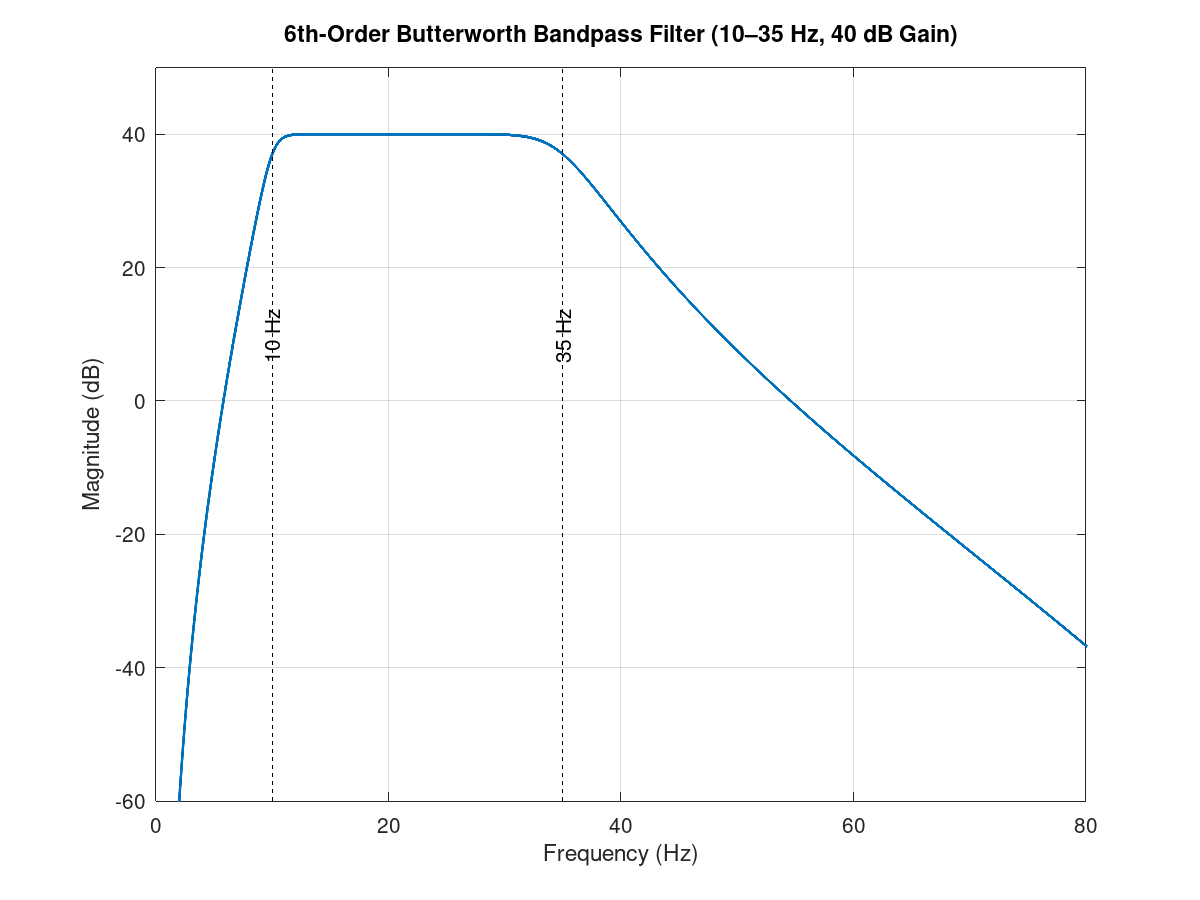
\includegraphics[width=14cm]{src/images/figures/6th_butterworth.png}
	\caption{6th-order Butterworth band pass filter’s frequency response}
	\label{bandpass}
\end{figure}

\section{Microcontroller Based Data Acquisition and Communication}
The microcontroller based data acquisition block will be used to convert the conditioned analog EEG signal to its corresponding digital equivalent which can then be used for real-time processing. The conditioned EEG signal will have the required frequency components after going through the instrumentation amplification and analog filtering blocks, but will still be a continuous time signal. This continuous time signal is fed to the internal ADC of the microcontroller, where the analog signal is converted to its digital counterpart by sampling the signal uniformly with respect to time. Before this process, the signal is level shifted to its mid supply value so that it can be fed to the single supply ADC.

\subsection{Analog to Digital Converter (ADC)}
After the EEG signal is amplified and filtered, it is still an analog signal, meaning it is a continuous voltage that varies with time. However, our microcontroller and signal 
processing algorithms (like FFT) can only work with digital data. Therefore, the signal must be converted from analog to digital, which is done using an Analog to Digital Converter (ADC). 

The filtered EEG signal (in microvolts, now amplified to millivolts/volts) is fed to the ADC input of the microcontroller. The ADC samples the EEG signal at a fixed 
sampling frequency (e.g., 256 Hz or 512 Hz), which is sufficient to capture EEG frequencies (0.5 – 40 Hz). Instead of a continuous waveform, we now have discrete time voltage values. 

The ADC used by our microcontroller is Successive Approximation Register(SAR) ADC. SAR ADC is a type of analog to digital converter that converges digital value towards input signal after every iteration by binary search. Here the search is done by comparing the current digital value in register with input value via DAC and makes a decision to step up or step down the digital value depending on the result of comparision. The digital value is updated from most significant bit to least significant bit. 

\begin{figure}[H]
	\centering
	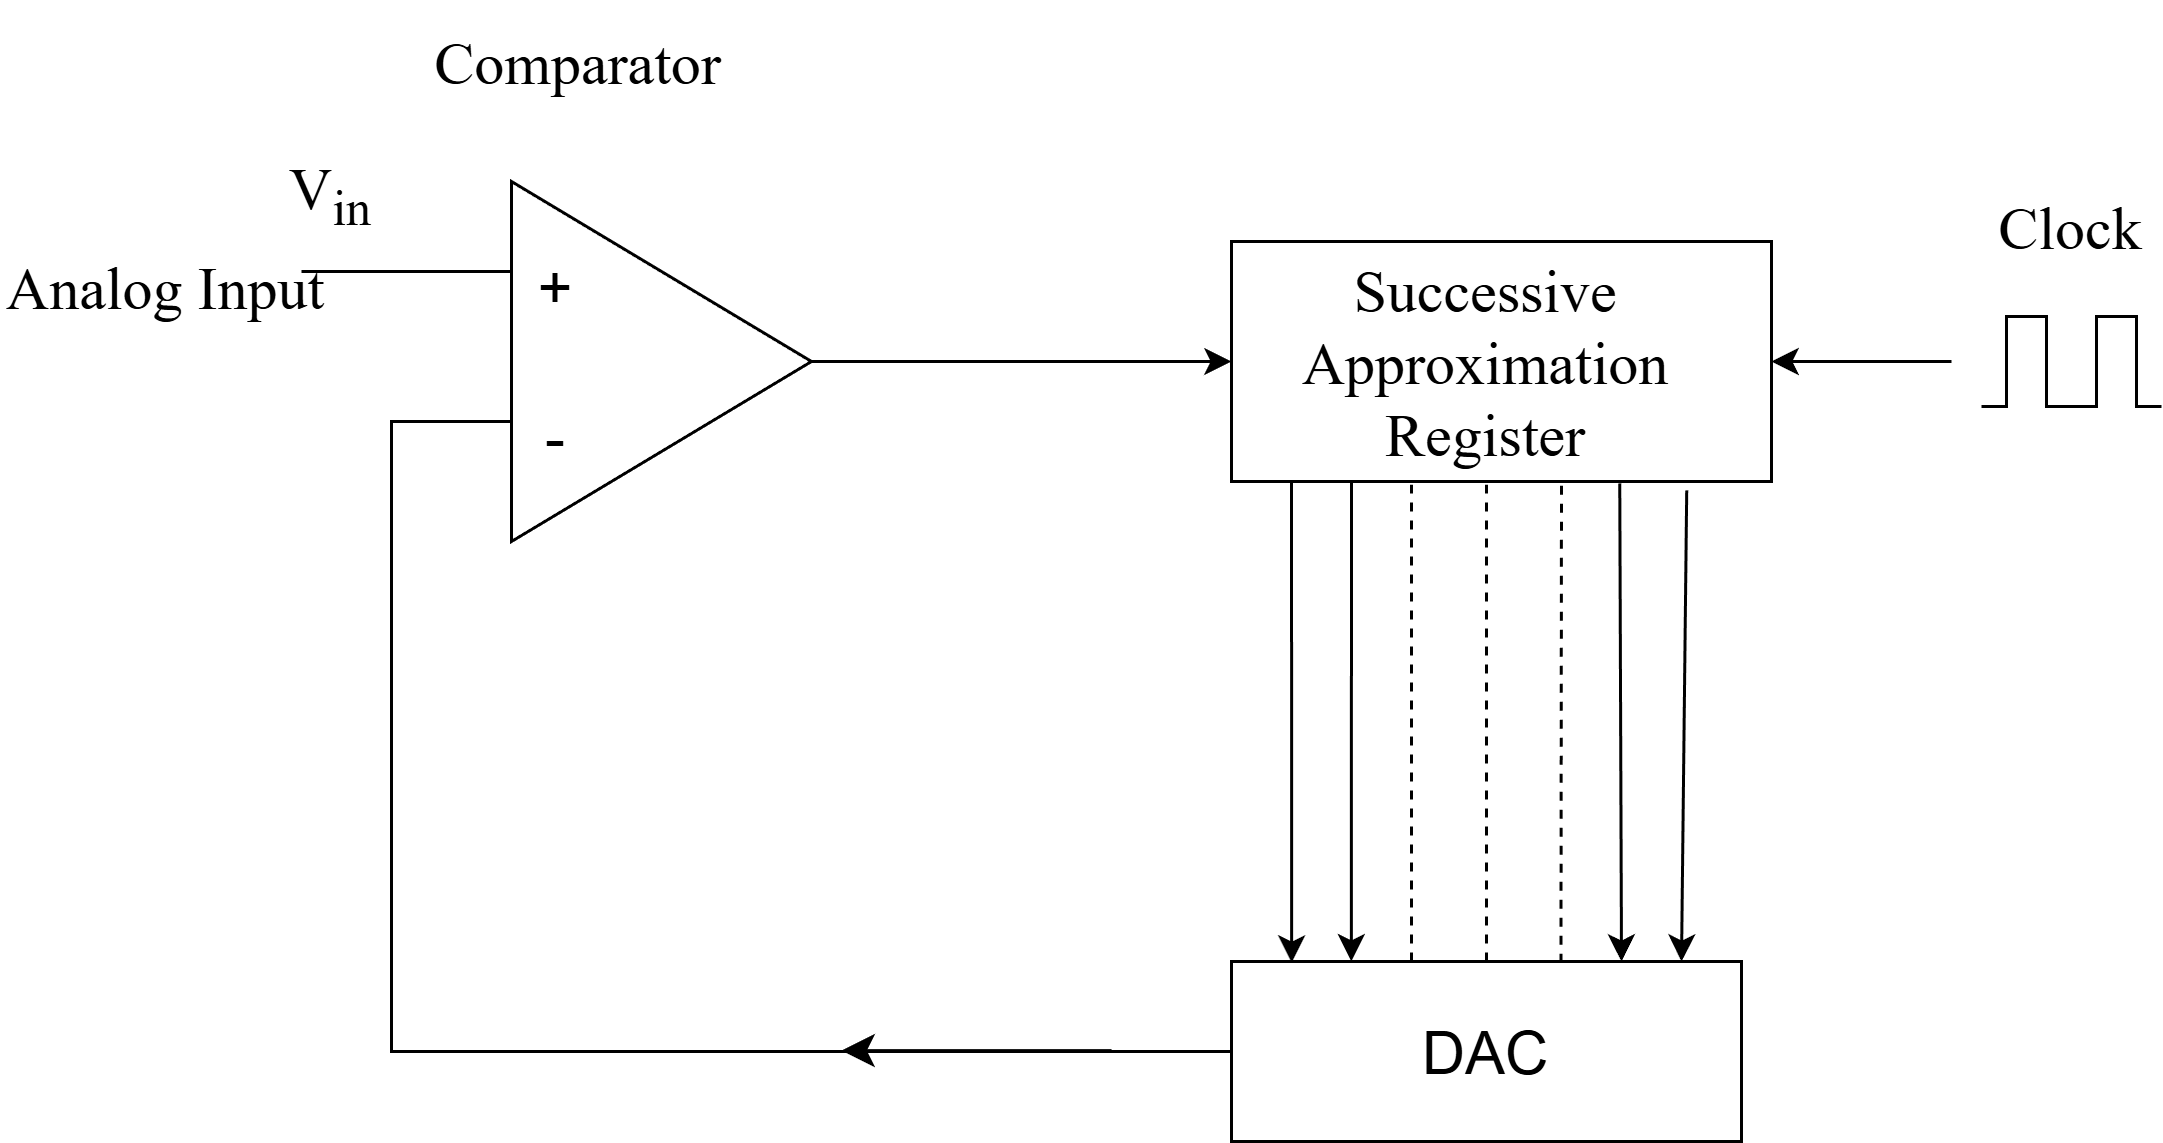
\includegraphics[width = 13.5cm, height=7.5cm]{src/images/figures/sar3.png}
\caption{Successive Approximation Register(SAR) ADC}
\label{Successive Approximation Register(SAR) ADC}
\end{figure}

\section{Arduino Timer Specifications}

Arduino boards, such as the Arduino Uno, feature built-in hardware timers that provide precise time measurement, event counting, and pulse generation. The key specifications of these timers are as follows:

\renewcommand{\labelitemi}{$\bullet$}
\renewcommand{\labelitemii}{$\bullet$}

\begin{itemize}
	\item \textbf{Timer Types:}
	\begin{itemize}
		\item 8-bit timers: Timer0, Timer2
		\item 16-bit timer: Timer1
	\end{itemize}
	
	\item \textbf{Modes of Operation:}
	\begin{itemize}
		\item Normal mode (simple counting)
		\item CTC (Clear Timer on Compare Match) mode
		\item PWM (Pulse Width Modulation) modes
	\end{itemize}
	
	\item \textbf{Clock Source:}  
	Each timer increments based on the system clock (16 MHz on Arduino Uno), optionally divided by a configurable prescaler (1, 8, 64, 256, 1024), allowing flexible timing intervals.
	
	\item \textbf{Interrupt Capabilities:}  
	Timers can generate interrupts on compare match, overflow, or external events, enabling precise periodic execution of code.
	
	\item \textbf{Resolution:}
	\begin{itemize}
		\item 8-bit timers: counts from 0 to 255
		\item 16-bit timer: counts from 0 to 65535
	\end{itemize}
	
	\item \textbf{Applications:}
	\begin{itemize}
		\item Generating precise delays and periodic signals
		\item Measuring time intervals
		\item Counting external pulses or events
		\item Producing PWM signals for motor and LED control
	\end{itemize}
\end{itemize}

\noindent These timers act as hardware counters, providing high accuracy and reliability for time sensitive tasks without relying on software delays.


\section{Frequency Domain Analysis Using Fast Fourier Transform (FFT)}
The digital data is now ready for processing. But the signal is in time domain i.e the signal shows voltage vs time. Brain rhythms (alpha, beta, etc.) are hidden inside the signal. So, the problem is, from the time domain signal alone, we cannot clearly separate brain waves by frequency. For that we need to convert the EEG signals from time domain to frequency domain. And a fourier transform allows us to do that. 
\begin{equation}
	F(\omega) = \int_{-\infty}^{\infty} x(t)\, e^{-j \omega t} \, dt
\end{equation}
where:\\
x(t): The original function or signal in the time domain.\\
$F(\omega)$: The transformed function in the frequency domain.\\
$\omega$: Angular frequency.\\
$e^{-j \omega t}$: A complex exponent representing sinusoidal components.
\section{Discrete Fourier Transform (DFT) and Fast Fourier Transform (FFT)}
The sampled data is discrete, not continuous. And that is why we use discrete fourier transform since the regular fourier transform is for continuous signals. The Discrete Fourier Transform (DFT) is used to convert our discrete time signal from the time domain into its frequency domain representation. It directly computes the frequency components using the DFT formula and requires a large number of computations. For an N point signal, DFT requires $O(N^2)$ complex multiplications, which makes it computationally slow for large data sets.\\The DFT of x[n] is mathematically defined as\\
\begin{equation}
	X[k] = \sum_{n=0}^{N-1} x[n]\; e^{-j \frac{2\pi k n}{N}},\\
	\quad k = 0,1,2,\ldots, N-1
\end{equation}
where,\\
k: index for output frequency component\\
X[k]: the complex frequency domain coefficient corresponding to the k-th frequency\\
N: total number of samples \\
n: the index for sample ranging from 0 to N-1 
x[n]:  n-th sample\\

The Fast Fourier Transform (FFT) is not a different transform but an efficient algorithm used to compute the Discrete Fourier Transform (DFT). FFT exploits the symmetry and periodicity properties of the DFT to reduce the number of calculations. Using FFT, the computational complexity is reduced from $O(N^2)$ to $O(N \log N)$, making it much faster and suitable for real-time signal processing applications such as EEG, ECG, image processing, and communication systems.

The FFT algorithm calculates the frequency components using a computational complexity of $O(N\log N)$, and this makes it possible to process the EEG signals in real-time. The magnitude of the FFT output either $|X[k]|$ or the power spectrum $|X[k]|^2$ shows the magnitude of each frequency component within the EEG signal. Through the power spectrum distribution in different frequency bands, including the beta frequency band (12-30 Hz), one can easily detect whether there are certain brain rhythms within the EEG signals. Therefore, the FFT algorithm converts the time domain EEG signals into frequency domain EEG signals.

\section{CORDIC Algorithm}
As we were implementing FFT algorithm, the need of using sine and cosine trigonometric function became inevitable. Using regular built-in library available is expensive for computation for our 16MHz Arduino micro-controller. So, we decided to adopt CORDIC algorithm to create our custom function which is tuned according to our need of accuracy trading off with the computation as accuracy is disposable since it is not our main concern.

The CORDIC algorithm (COordinate Rotation DIgital Computer) is an efficient iterative method useful to compute various mathematical functions, especially trigonometric, hyperbolic, exponential, logarithmic functions, square roots, and vector rotations using only shift and add operations.


The CORDIC (COordinate Rotation DIgital Computer) algorithm computes vector rotations using only iterative shift-and-add operations. 
A vector $(x, y)$ is rotated by breaking the desired rotation into a sequence of smaller micro-rotations:

\begin{equation}
	\theta_i = \tan^{-1}(2^{-i})
\end{equation}

Each iteration performs a rotation by $\pm \theta_i$, which can be implemented using only arithmetic shifts and additions.

The standard rotation equations are:

\begin{equation}
	x' = x \cos\theta - y \sin\theta
\end{equation}
\begin{equation}
	y' = x \sin\theta + y \cos\theta
\end{equation}

CORDIC rewrites these using the identity $\tan\theta \approx 2^{-i}$, allowing multiplication by powers of two to be replaced with bit shifts.

The iterative update equations become:

\begin{align}
	x_{i+1} &= x_i - d_i \cdot y_i \cdot 2^{-i} \\
	y_{i+1} &= y_i + d_i \cdot x_i \cdot 2^{-i} \\
	z_{i+1} &= z_i - d_i \cdot \tan^{-1}(2^{-i})
\end{align}
where $d_i \in \{-1, +1\}$ determines the direction of rotation.

\subsection{Scaling Factor}

Each micro-rotation introduces a scaling effect on the vector magnitude. After $n$ iterations, the accumulated scale factor is:

\begin{equation}
	K_n = \prod_{i=0}^{n-1} \frac{1}{\sqrt{1 + 2^{-2i}}}
\end{equation}

Thus, the true magnitude must be corrected as:

\begin{equation}
	\begin{bmatrix}
		x_{\text{final}} \\
		y_{\text{final}}
	\end{bmatrix}
	=
	K_n
	\begin{bmatrix}
		x_n \\
		y_n
	\end{bmatrix}
\end{equation}

where $K_n$ is typically precomputed for a given number of iterations.

\section{Twiddle Factor Computation Under Recurrence}
Twiddle factors in the Fast Fourier Transform (FFT) are defined as:

\begin{equation}
	W_N^k = e^{-j \frac{2\pi k}{N}}
\end{equation}

where \(N\) is the FFT size, \(k\) is the index, and \(j = \sqrt{-1}\).

Instead of computing each value using sine and cosine, FFT uses a recurrence approach. Define the general twiddle factor:

\begin{equation}
	W_N = e^{-j \frac{2\pi}{N}}
\end{equation}

Then any twiddle factor can be written as:
\begin{equation}
	W_N^k = (W_N)^k
\end{equation}

From this, we obtain the recurrence relation:
\begin{equation}
	W_N^{k+1} = W_N^k \cdot W_N
\end{equation}

This means each successive twiddle factor is obtained by multiplying the previous one by a fixed complex constant \(W_N\), which corresponds to a constant rotation on the complex unit circle:

\begin{equation}
	e^{j\theta} \cdot e^{j\Delta\theta} = e^{j(\theta + \Delta\theta)}
\end{equation}

Thus:
\begin{equation}
	W \leftarrow W \cdot W_N
\end{equation}

generates all required roots of unity efficiently without recomputing sine and cosine values.

\begin{figure}[H]
	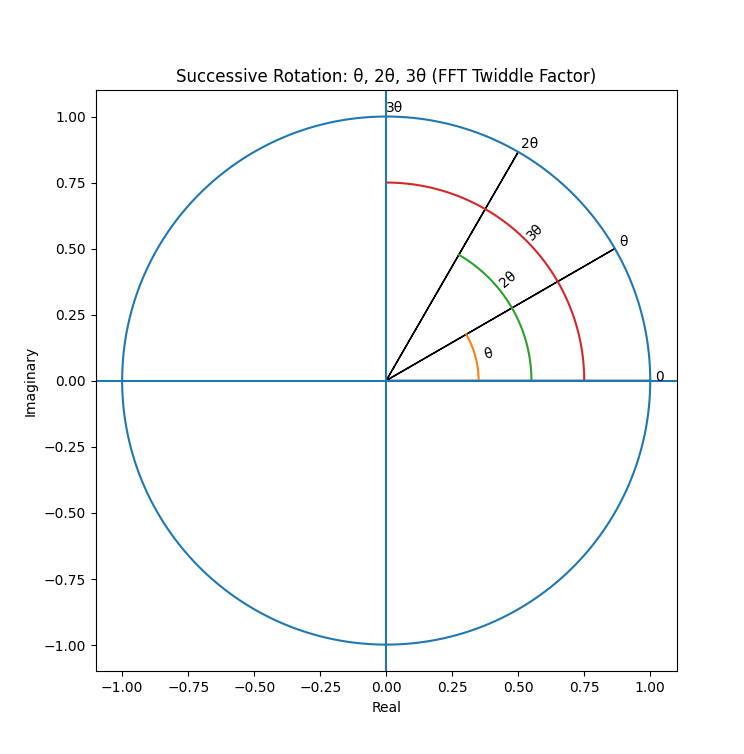
\includegraphics[width=14cm]{src/images/figures/rotation.png}
	\caption{Twiddle Factor Computation Under Unit Circle Rotation}
	\label{twiddle}
\end{figure}


\section{Windowing -- Hann Window}

When performing a Fourier transform, the signal taken for sampling is finite, with no guarantee of perfect start and end points of the waveform, which causes inaccuracies in frequency analysis. Due to this, spectral energy from high-energy frequencies spreads into neighboring frequencies. This phenomenon is known as spectral leakage.

Although spectral leakage cannot be completely eliminated, it can be reduced using windowing techniques. Windowing reduces spectral leakage by smoothing the signal at its boundaries before transforming it from the time domain to the frequency domain.

In this project, the Hann window is used to reduce spectral leakage before transforming the EEG signal. The Hann window smooths abrupt signal transitions by gradually reducing the signal amplitude to zero at the edges, making it suitable for EEG frequency analysis. The Hann window is defined as:
\begin{equation}
w(n) = \frac{1}{2}\left(1 - \cos\left(\frac{2\pi n}{N-1}\right)\right), \quad n = 0, 1, 2, \ldots, N-1
\end{equation}

\begin{figure}[H]
	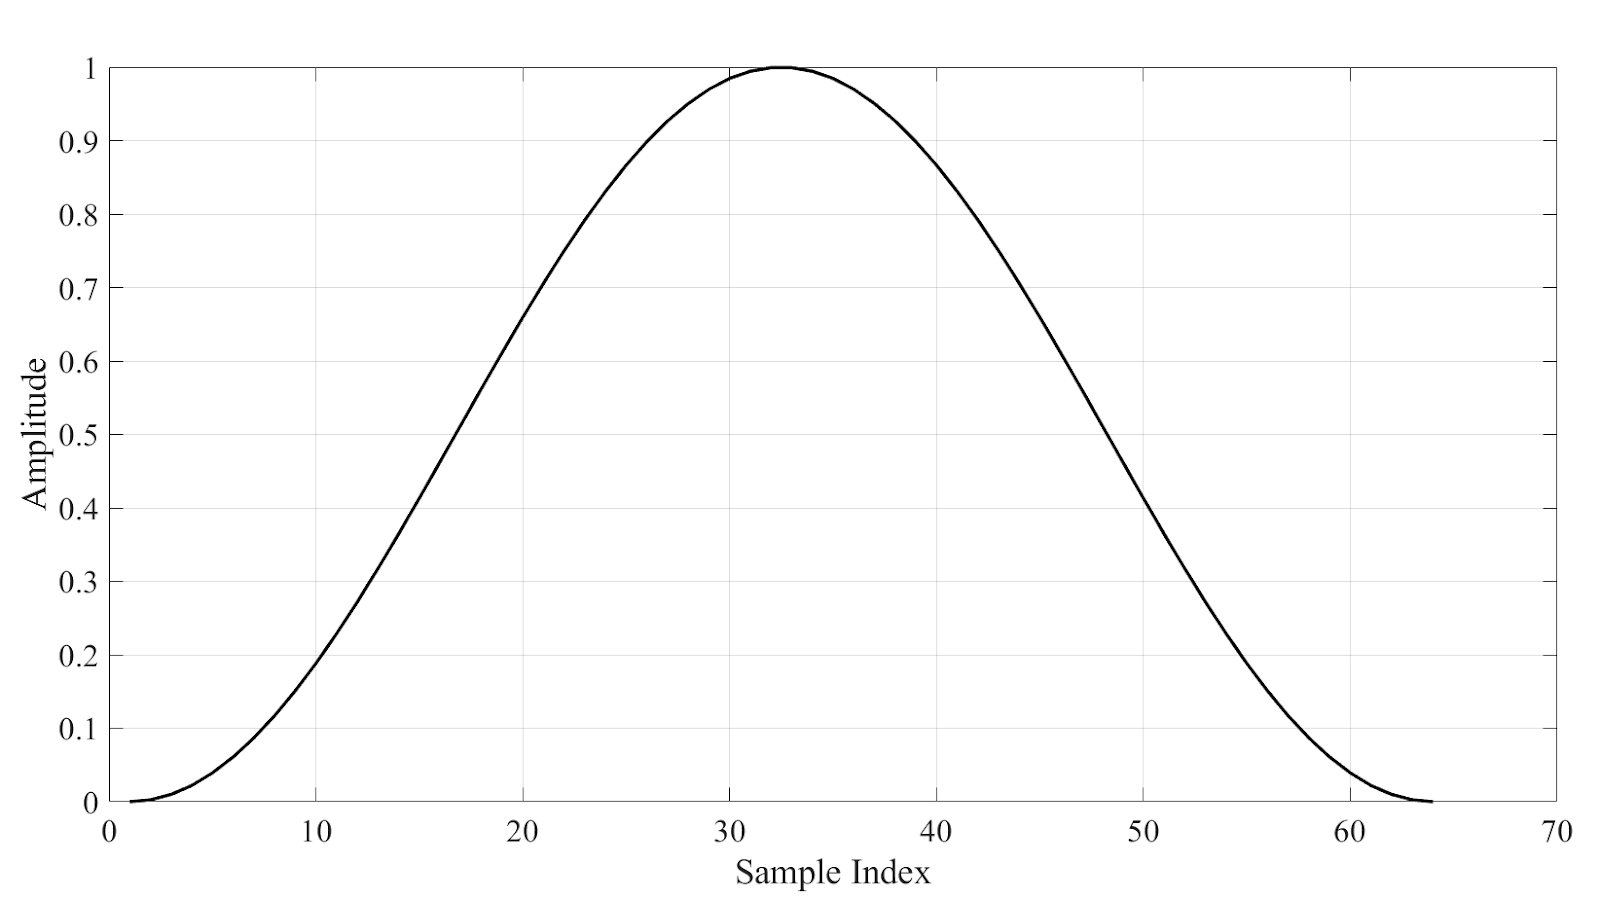
\includegraphics[width=14cm]{src/images/figures/hann.png}
	\caption{Hann Window}
	\label{hann}
\end{figure}

\begin{figure}[H]
	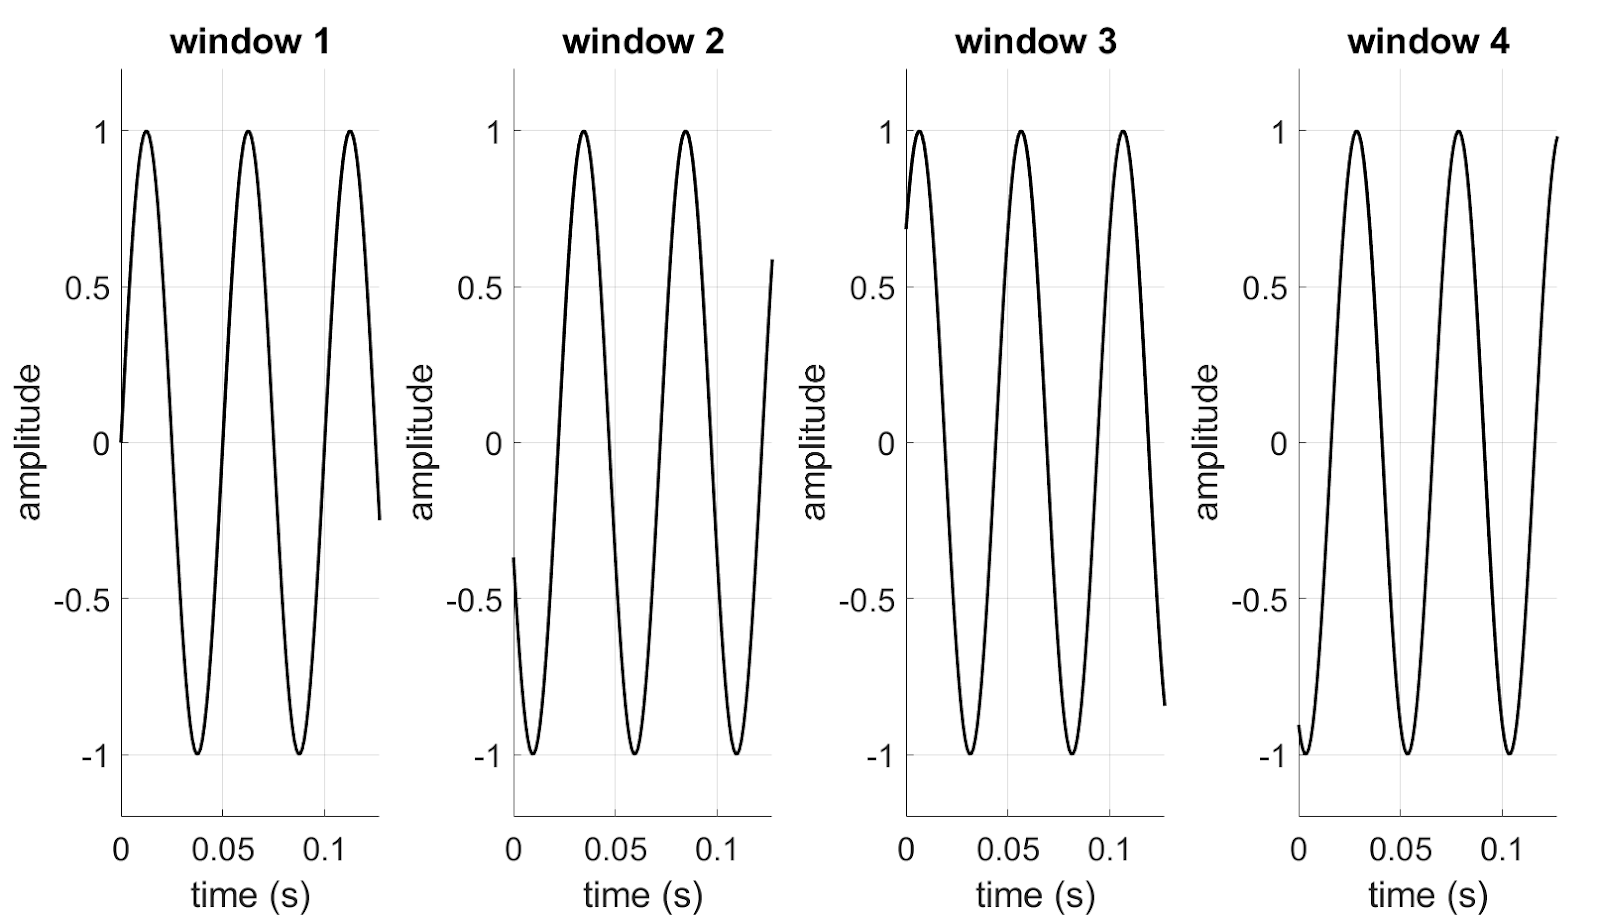
\includegraphics[width=14cm]{src/images/figures/discontinuous_wave.png}
	\caption{Discontinuous wave during window transition}
	\label{discontinuous}
\end{figure}

\begin{figure}[H]
	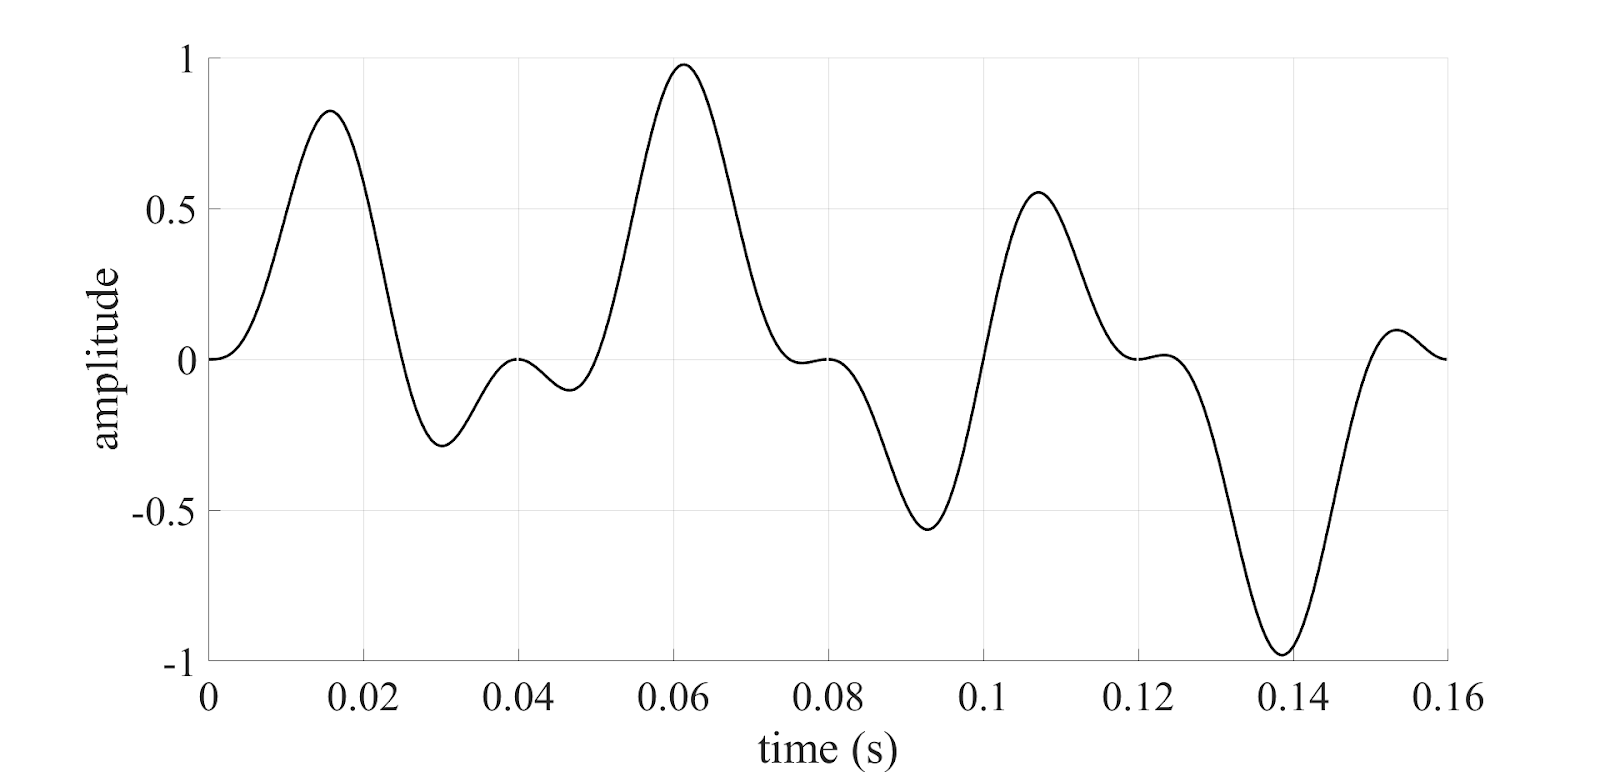
\includegraphics[width=14cm]{src/images/figures/continuity_hann.png}
	\caption{Continuity due to Hann window application on \ref{discontinuous}}
	\label{hann_continuous}
\end{figure}

\section{Processing After Fast Fourier Transform (FFT)}

The output from the Fast Fourier Transform is used to transform the digitized EEG signal from the time domain to the frequency domain. From the output of the Fast Fourier Transform, it is possible to obtain information on the distribution of power in the frequency components of the signal. The power for each frequency is obtained by using the real and imaginary components of the output from the FFT.

The relevant features in the frequency domain are obtained by computing power within certain frequency ranges. Power in the lower frequency range indicates eye blink activity while that in higher frequency ranges such as the beta range (13-30 Hz) indicate focused mental activity. The system uses the computed band-wise power values as its features.

The selected features are compared against pre-defined threshold values in the microcontroller. When the power value for the blink related frequency range exceeds the blink threshold, the system classifies the input signal as eye blink. On the other hand, when the power value for the focus related frequency range exceeds the focus threshold, the system classifies the signal as focus. Accordingly, the system generates commands; blink command for traversing the keys and focus command for key selection.